\documentclass{scrartcl}

\usepackage[top=3cm, bottom=4cm, left=2cm, right=2cm]{geometry}
\usepackage[ngerman]{babel}
\usepackage{hyperref}
\usepackage{tcolorbox}
\usepackage{csquotes}
\usepackage{fontawesome}

% TODO:
\definecolor{hintboxcolor}{rgb}{0.5,0.5,0.5}
\definecolor{myurlcolor}{rgb}{0.3,0.3,0.6}

\hypersetup{
	colorlinks,
	urlcolor=myurlcolor
}

\title{\vspace{-2cm}Instructions for submitting the programming tasks via GitLab}
% TODO:
%\subtitle{}
%\author{}
%\date{}

\begin{document}
	\maketitle
	
	\begin{enumerate}
		\item Open the GitLab and log in with your university account data:
		
		\vfill
		
		\url{<YOUR_GITLAB_URL>} % TODO
		
		\vfill
	
		\item You will now see an overview of the available programming tasks:
		
		\vfill
		
		\begin{figure}[h!]
			\centering
			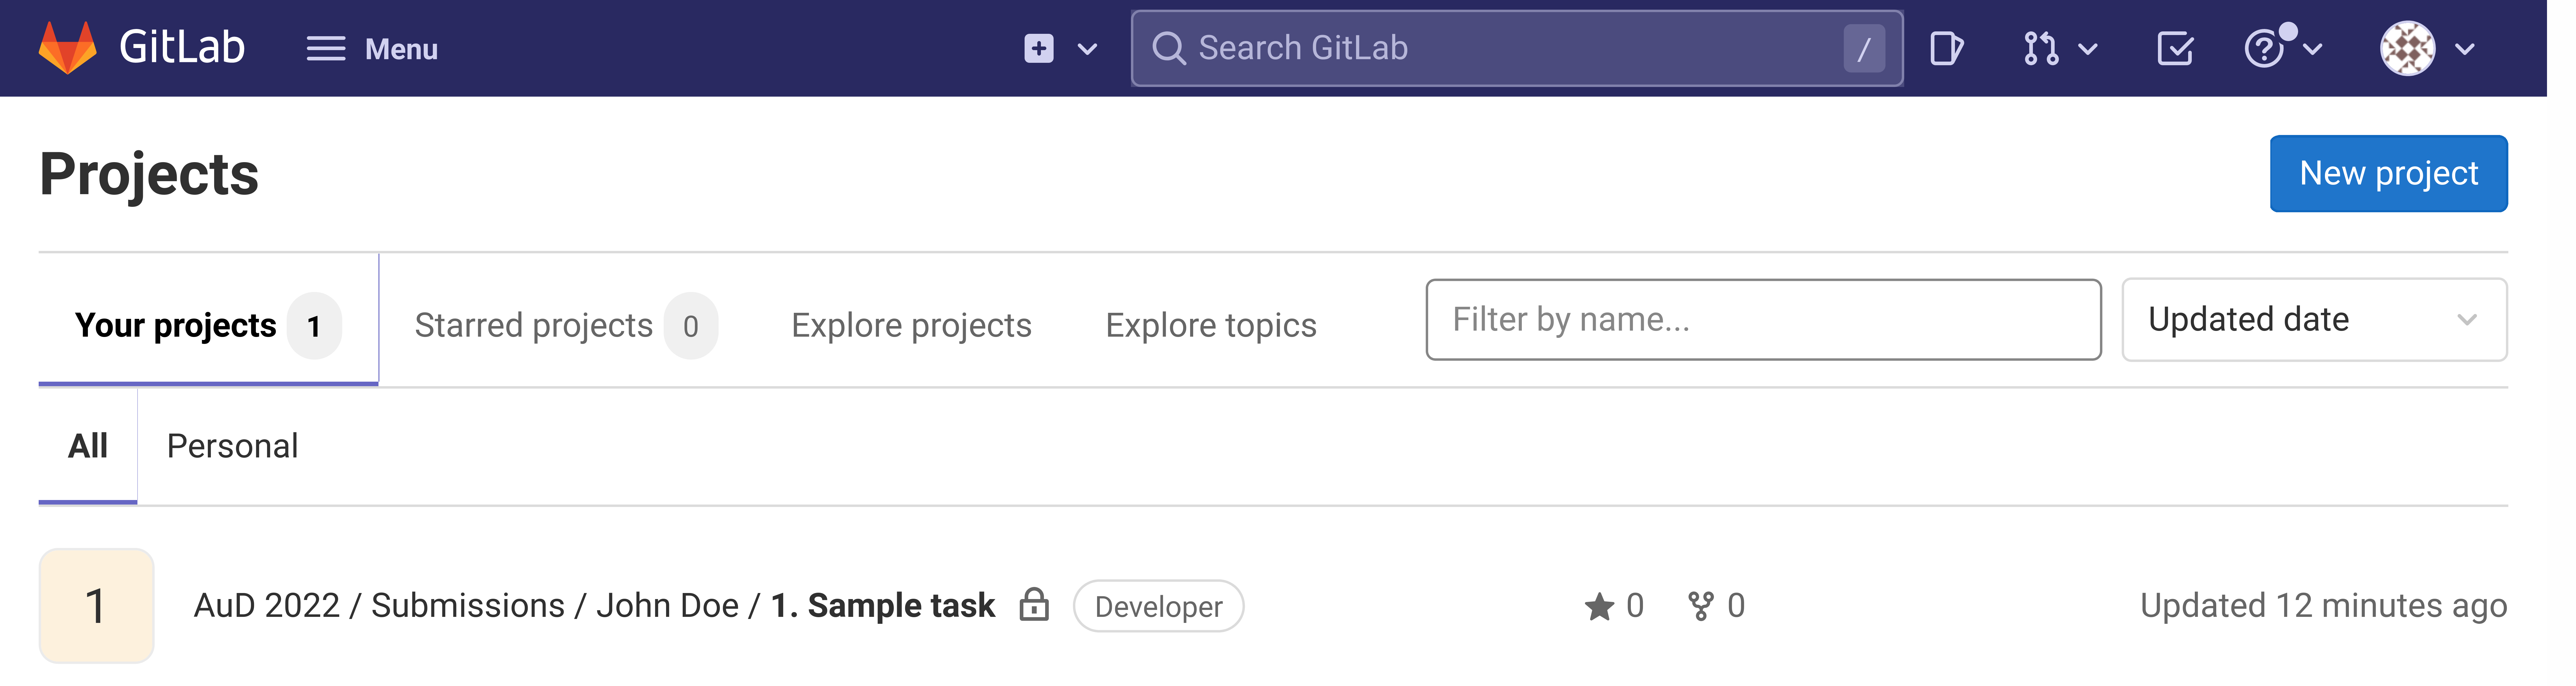
\includegraphics[width=0.9\textwidth]{img/en/screenshot-project-overview.png}
		\end{figure}
		
		\vfill

		Click on the programming task you want to work on.
		
		\vfill

		\begin{tcolorbox}[title=\faLightbulbO\space Hint,colbacktitle=hintboxcolor,colframe=hintboxcolor]
			If you have never used this GitLab before, you will not see the 1st programming task immediately after logging into your account. The task should appear within a few hours, max. 1 business day, so check back later.
		\end{tcolorbox}
		
		\vspace{6cm}
		
		\newpage
		
		\item You will now see a list of files that belong to the programming task, as well as the task description:
		
		\vfill
		
		\begin{figure}[h!]
			\centering
			\includegraphics[width=0.9\textwidth]{img/en/screenshot-project.png}
		\end{figure}
		
		\vfill
		
		Three files belong to each programming task:
		
		\begin{itemize}
			\item \texttt{README.md} contains the task definition.
			\item \texttt{StudentTestSuite.py} contains tests that you can use to check your solution before submitting it.
			\item \texttt{solution.py} contains the basic framework of the solution. Here you have to insert your implementation.
		\end{itemize}
	
		\vfill
		
		\item Download the files by clicking on the download icon \faDownload\space:
		
		\vfill
		
		\begin{figure}[h!]
			\centering	
			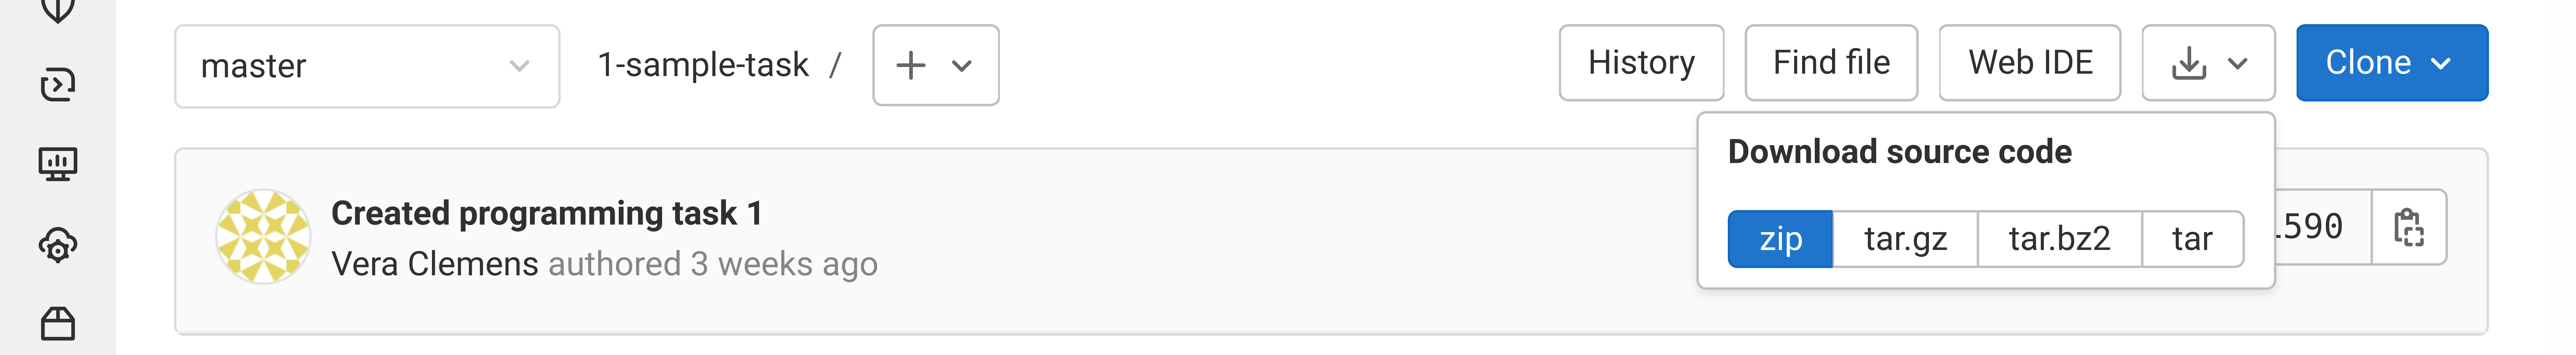
\includegraphics[width=0.9\textwidth]{img/en/screenshot-download.png}
		\end{figure}
		
%		\vfill
%		
%		\begin{tcolorbox}[title=\faLightbulbO\space Hint,colbacktitle=hintboxcolor,colframe=hintboxcolor]
%			You can also download the Git repository using the \enquote{Clone} button. Do this only if you have prior knowledge of Git and know what you are doing. We can't provide any support for this.
%		\end{tcolorbox}
		
		\vfill
		
		\pagebreak
		
		\item Now work on the programming task by developing your implementation in \texttt{solution.py}. In between you can always check if your solution works correctly for the example inputs by running the tests. To do this, open a terminal in the directory where your solution and test file are located and run:
		
		\vfill
		
		\texttt{python3 -m unittest StudentTestSuite.py}
		
		\vfill
		
		You will get an output telling you whether you pass all test cases or not.
		
		\vfill
		
		\item Once you think your implementation is correct, you can submit it to GitLab.
		
		\vfill
		
		\begin{tcolorbox}[title=\faExclamationCircle\space Caution,colbacktitle=red!75,colframe=red!75]
			\bfseries You have only 3 submission attempts for each programming task.

			Do not submit a solution that does not pass all test cases in the student test suite!
			
			Also, pay close attention to the general instructions in the assignment (do not use \texttt{import} or \texttt{input} statements, do not add code outside of the required functions,\ldots)!
		\end{tcolorbox}
	
		\vfill
	
		To do this, click \texttt{solution.py} in the file list. 

		Then click on \enquote{Replace}:
		
		\vfill
		
		
\includegraphics[width=0.9\textwidth]{img/screenshot-replace-button.png}
		
		\vfill
		
		Select your solution file for upload and then click \enquote{Replace file}:
		
		\vfill
		
		\begin{figure}[h!]
			\centering
			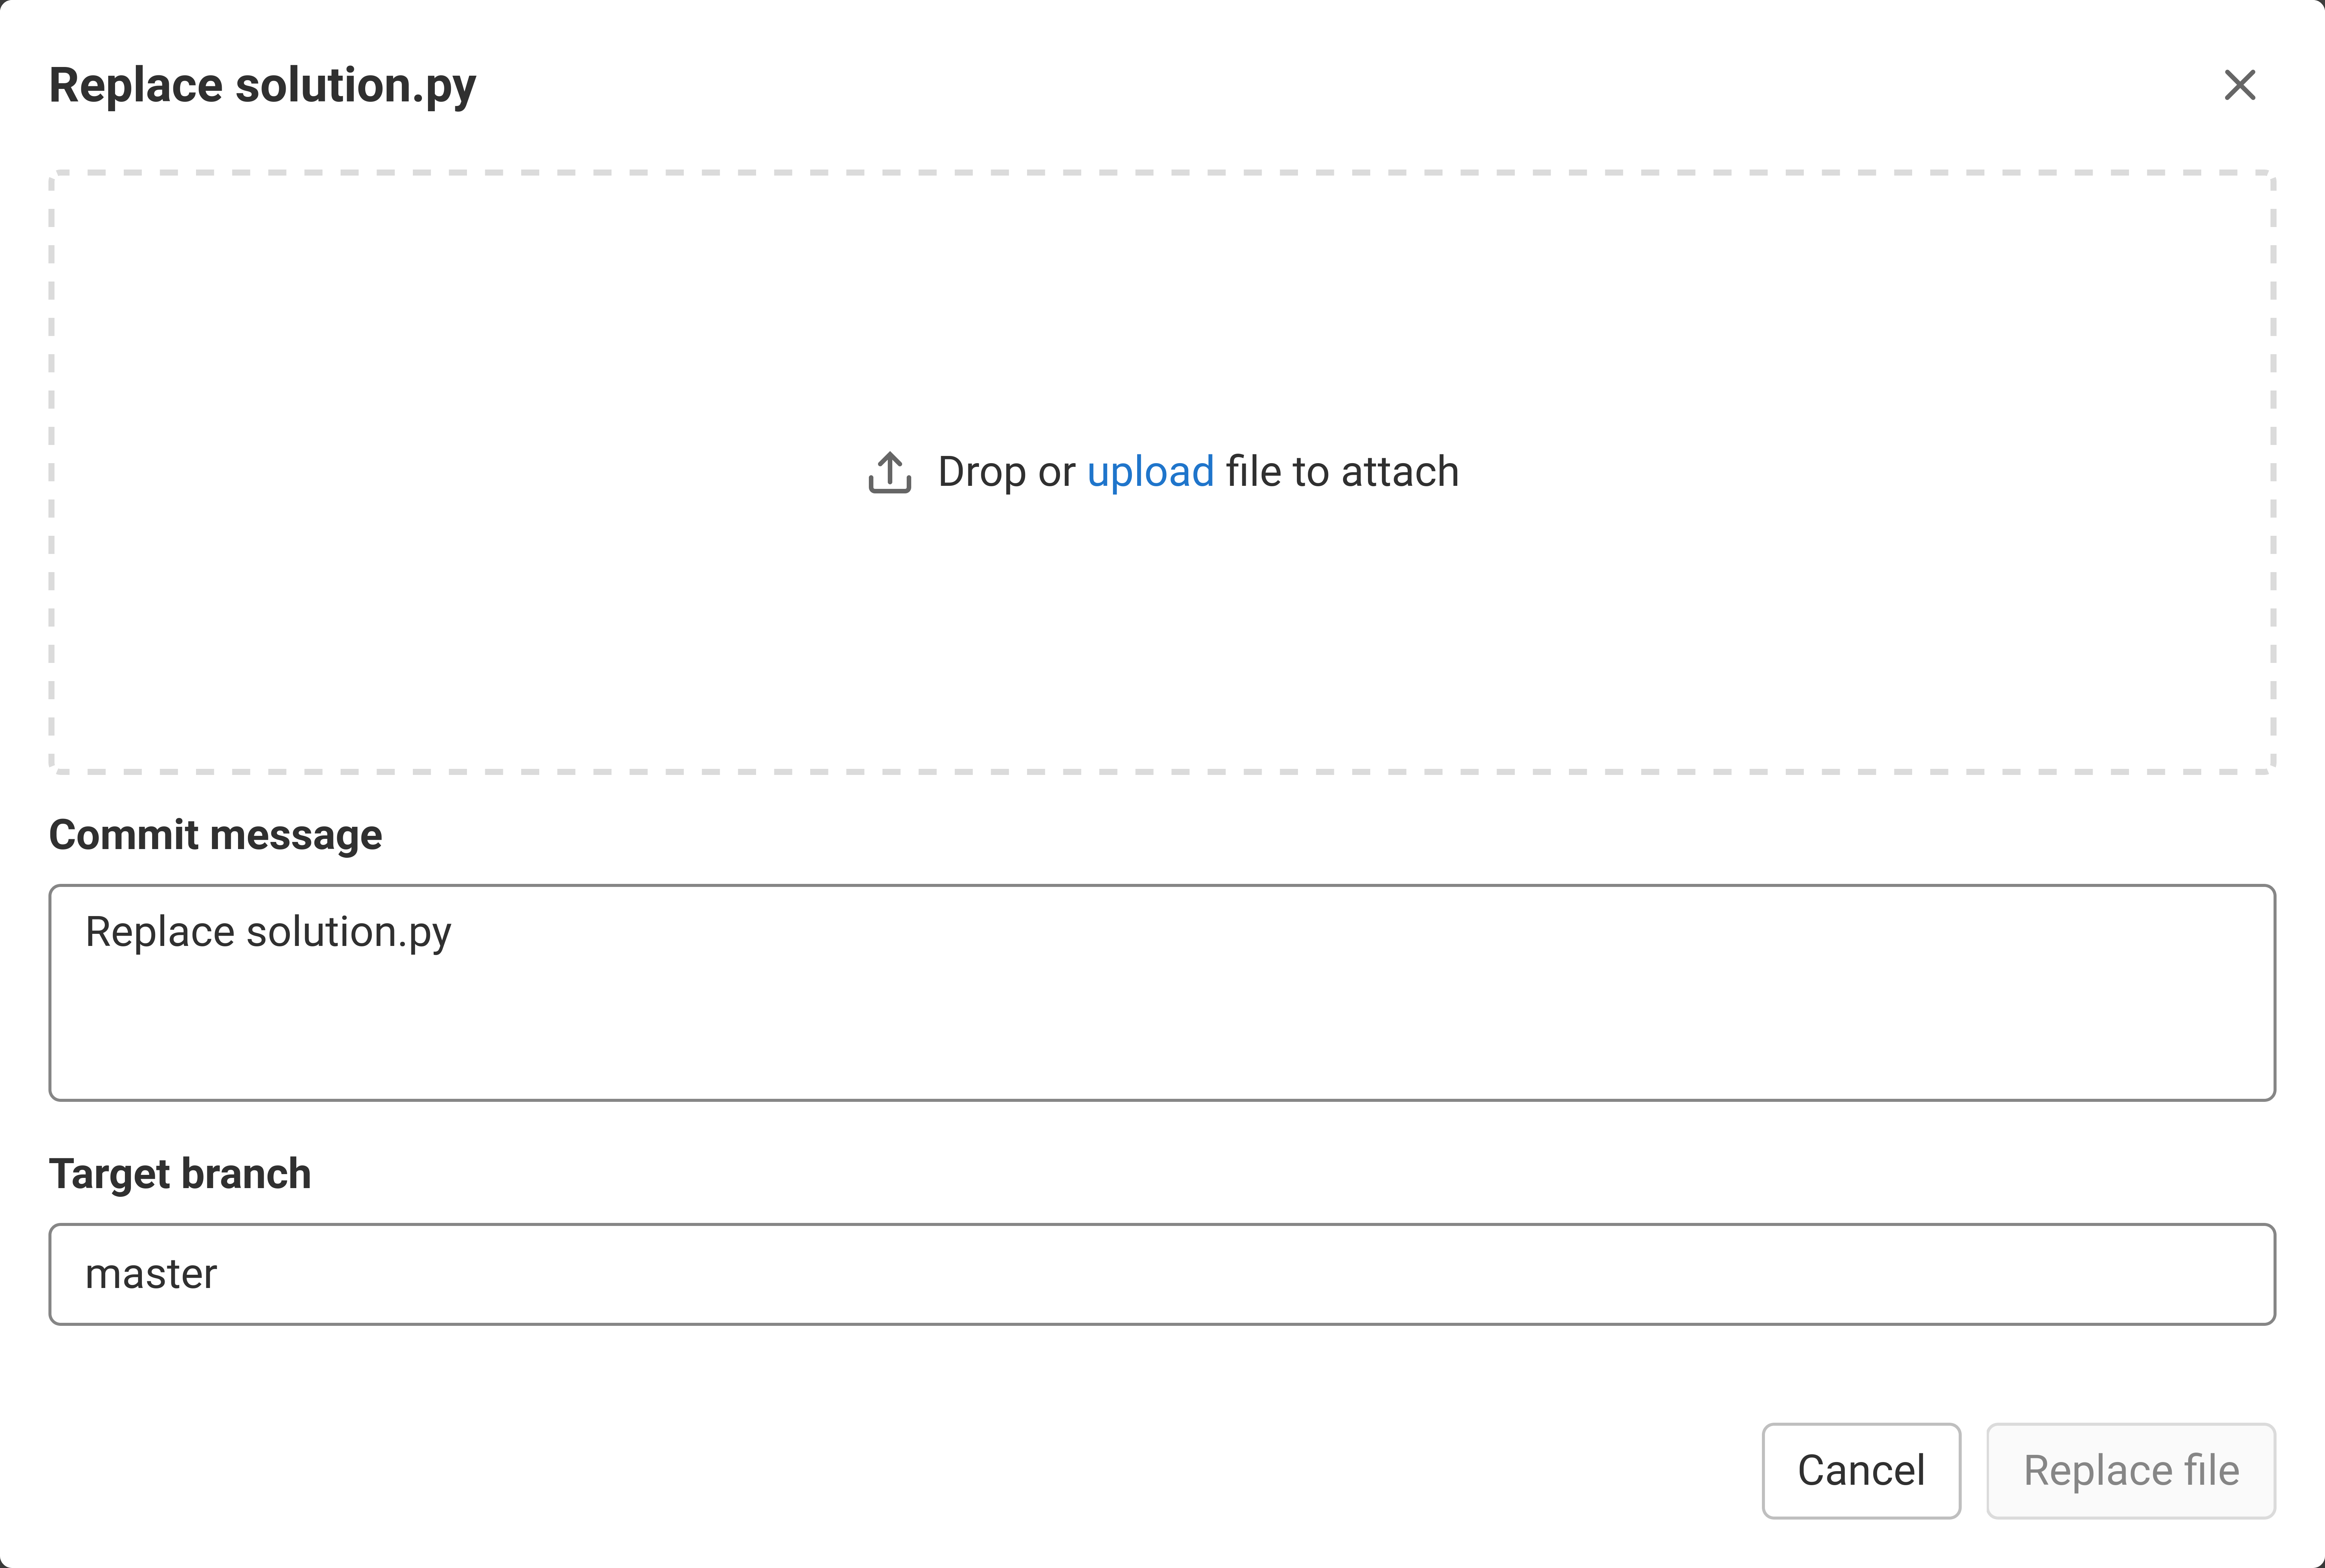
\includegraphics[width=0.75\textwidth]{img/screenshot-replace-dialog.png}
		\end{figure}
		
		\vfill
		
		You have successfully submitted your solution!
		
		\vfill
		
		\item Now your solution will be checked automatically. We use the student test suite, which is available to you, but in addition we also use other tests. We also check if you have followed the instructions in the assignment.

		To see the results of the check, click on the colorful icon next to your upload:
		
		\vfill
		
		\begin{figure}[h!]
			\centering
			
\includegraphics[width=0.9\textwidth]{img/screenshot-pipeline-icon.png}
		\end{figure}
		
		\vfill
		
		As long as the check is still running, the icon is a blue circle, after that either a green tick or a red cross.
		
		\vfill
		
		\item You can now see the results of the tests:
		
		\vfill
		
		\begin{figure}[h!]
			\centering
			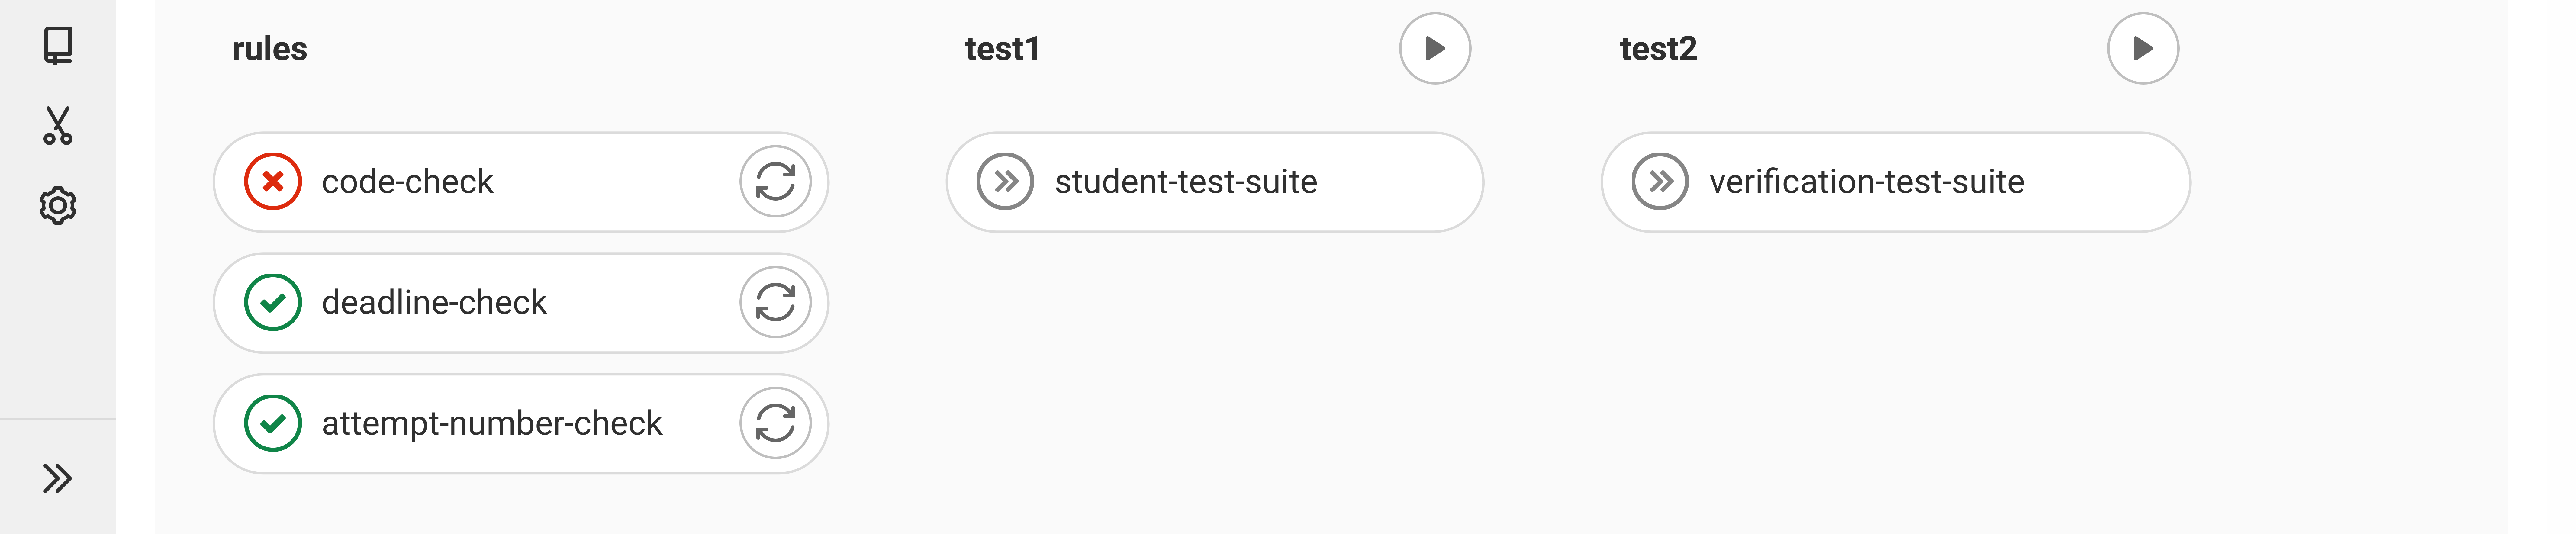
\includegraphics[width=0.9\textwidth]{img/en/screenshot-pipeline-results.png}
		\end{figure}
		
		\vfill
		
		Ideally all hooks are green. If not (as is the case here), your solution still has a bug. Click on the respective test to get a hint how to solve the error, e.g.:
		
		\vfill
		
		\begin{figure}[h!]
			\centering		
			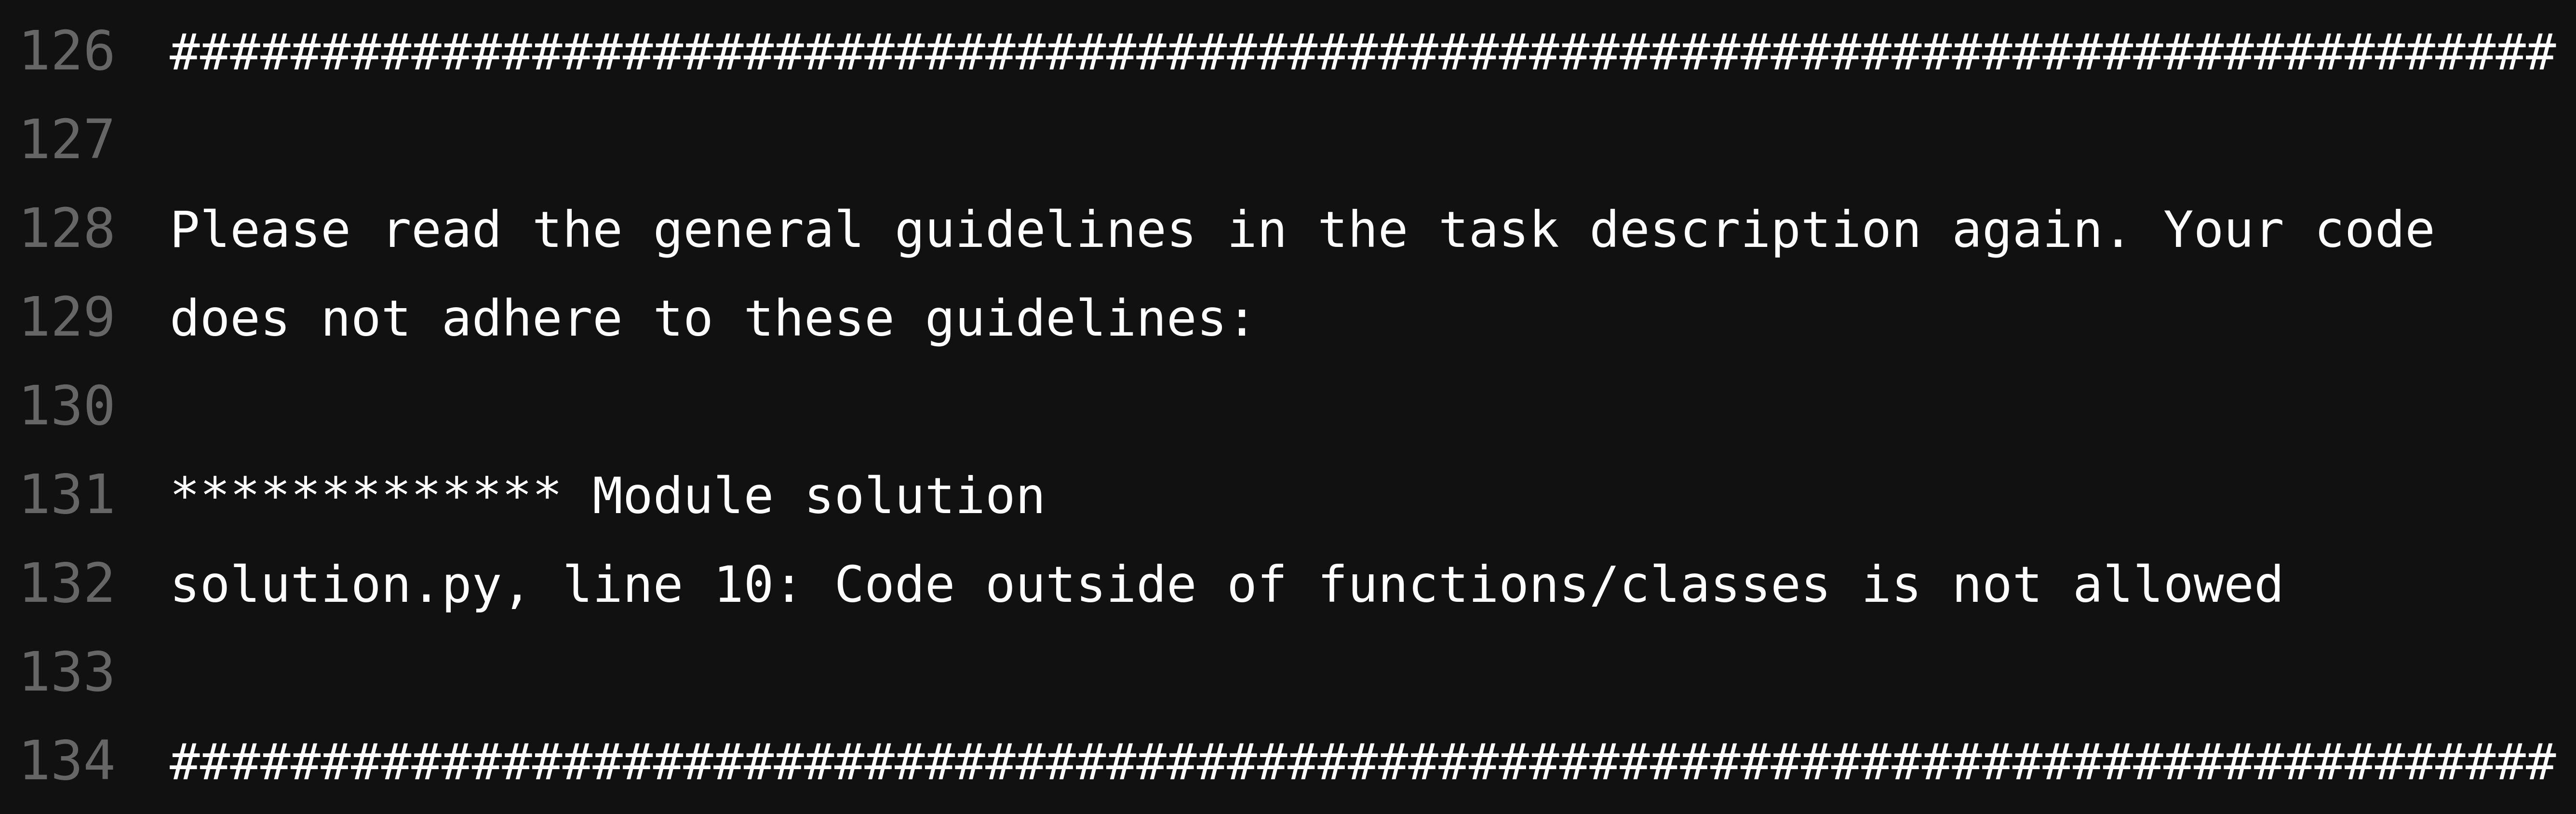
\includegraphics[width=0.75\textwidth]{img/en/screenshot-hint.png}
		\end{figure}
		
		\vfill
		
		\begin{tcolorbox}[title=\faLightbulbO\space Hint,colbacktitle=hintboxcolor,colframe=hintboxcolor]
			If you click on \enquote{attempt-number-check}, you will always be shown how many submission attempts you have left.
			Under \enquote{deadline-check}, you can see the remaining time until the deadline.
			
			\bfseries All submissions after the third attempt or after the deadline do not count.
		\end{tcolorbox}
	
		\vfill
		
		\item If you have any questions about GitLab or the programming assignments, make a post in the questions forum on Moodle.
		
		\vspace{1cm}
		
		{\Huge Good luck!}
	\end{enumerate}
\end{document}